\graphicspath{{./figs/chap2/}} % graphics location for this chapter

%--------------------------------------------------------------%
    % Begin Chapter
%--------------------------------------------------------------%
\chapter{Experimental Setup and Device Fabrication}\label{chap:two}
In this chapter the techniques needed in order to fabricate \ac{2D} transistors
are introduced and explained. Basic techniques such as the exfoliation of atomically thin \acp{TMD} crystals 
to more advanced techniques such as \ac{vdW} assembly of structures using various transfer methods are explored
in great detail. In addition, more general processes related to the fabrication of semiconductor devices
are explained as well. 
%--------------------------------------------------------------%
    % Crystal Synthesis
%--------------------------------------------------------------%
\section{Sample Preparation}\label{sec:sample_prep}

%--------------------------------------------------------------%
\subsection{Synthesis of Crystal Material}\label{subsec:crystal_synthesis}

%--------------------------------------------------------------%
    % Sample Prep
%--------------------------------------------------------------%
\section{Preparation of Atomically Thin Two-Dimensional Materials}\label{sec:prep_of_samples}

%--------------------------------------------------------------%
\subsection{Exfoliation of Atomically Thin Materials}\label{subsec:exfoliation}

%--------------------------------------------------------------%
\subsection{Characterization of Atomically Thin Materials}\label{subsec:exfoliation_characterization}
\begin{figure}[ht]
    \centering
    \subfloat[]{
        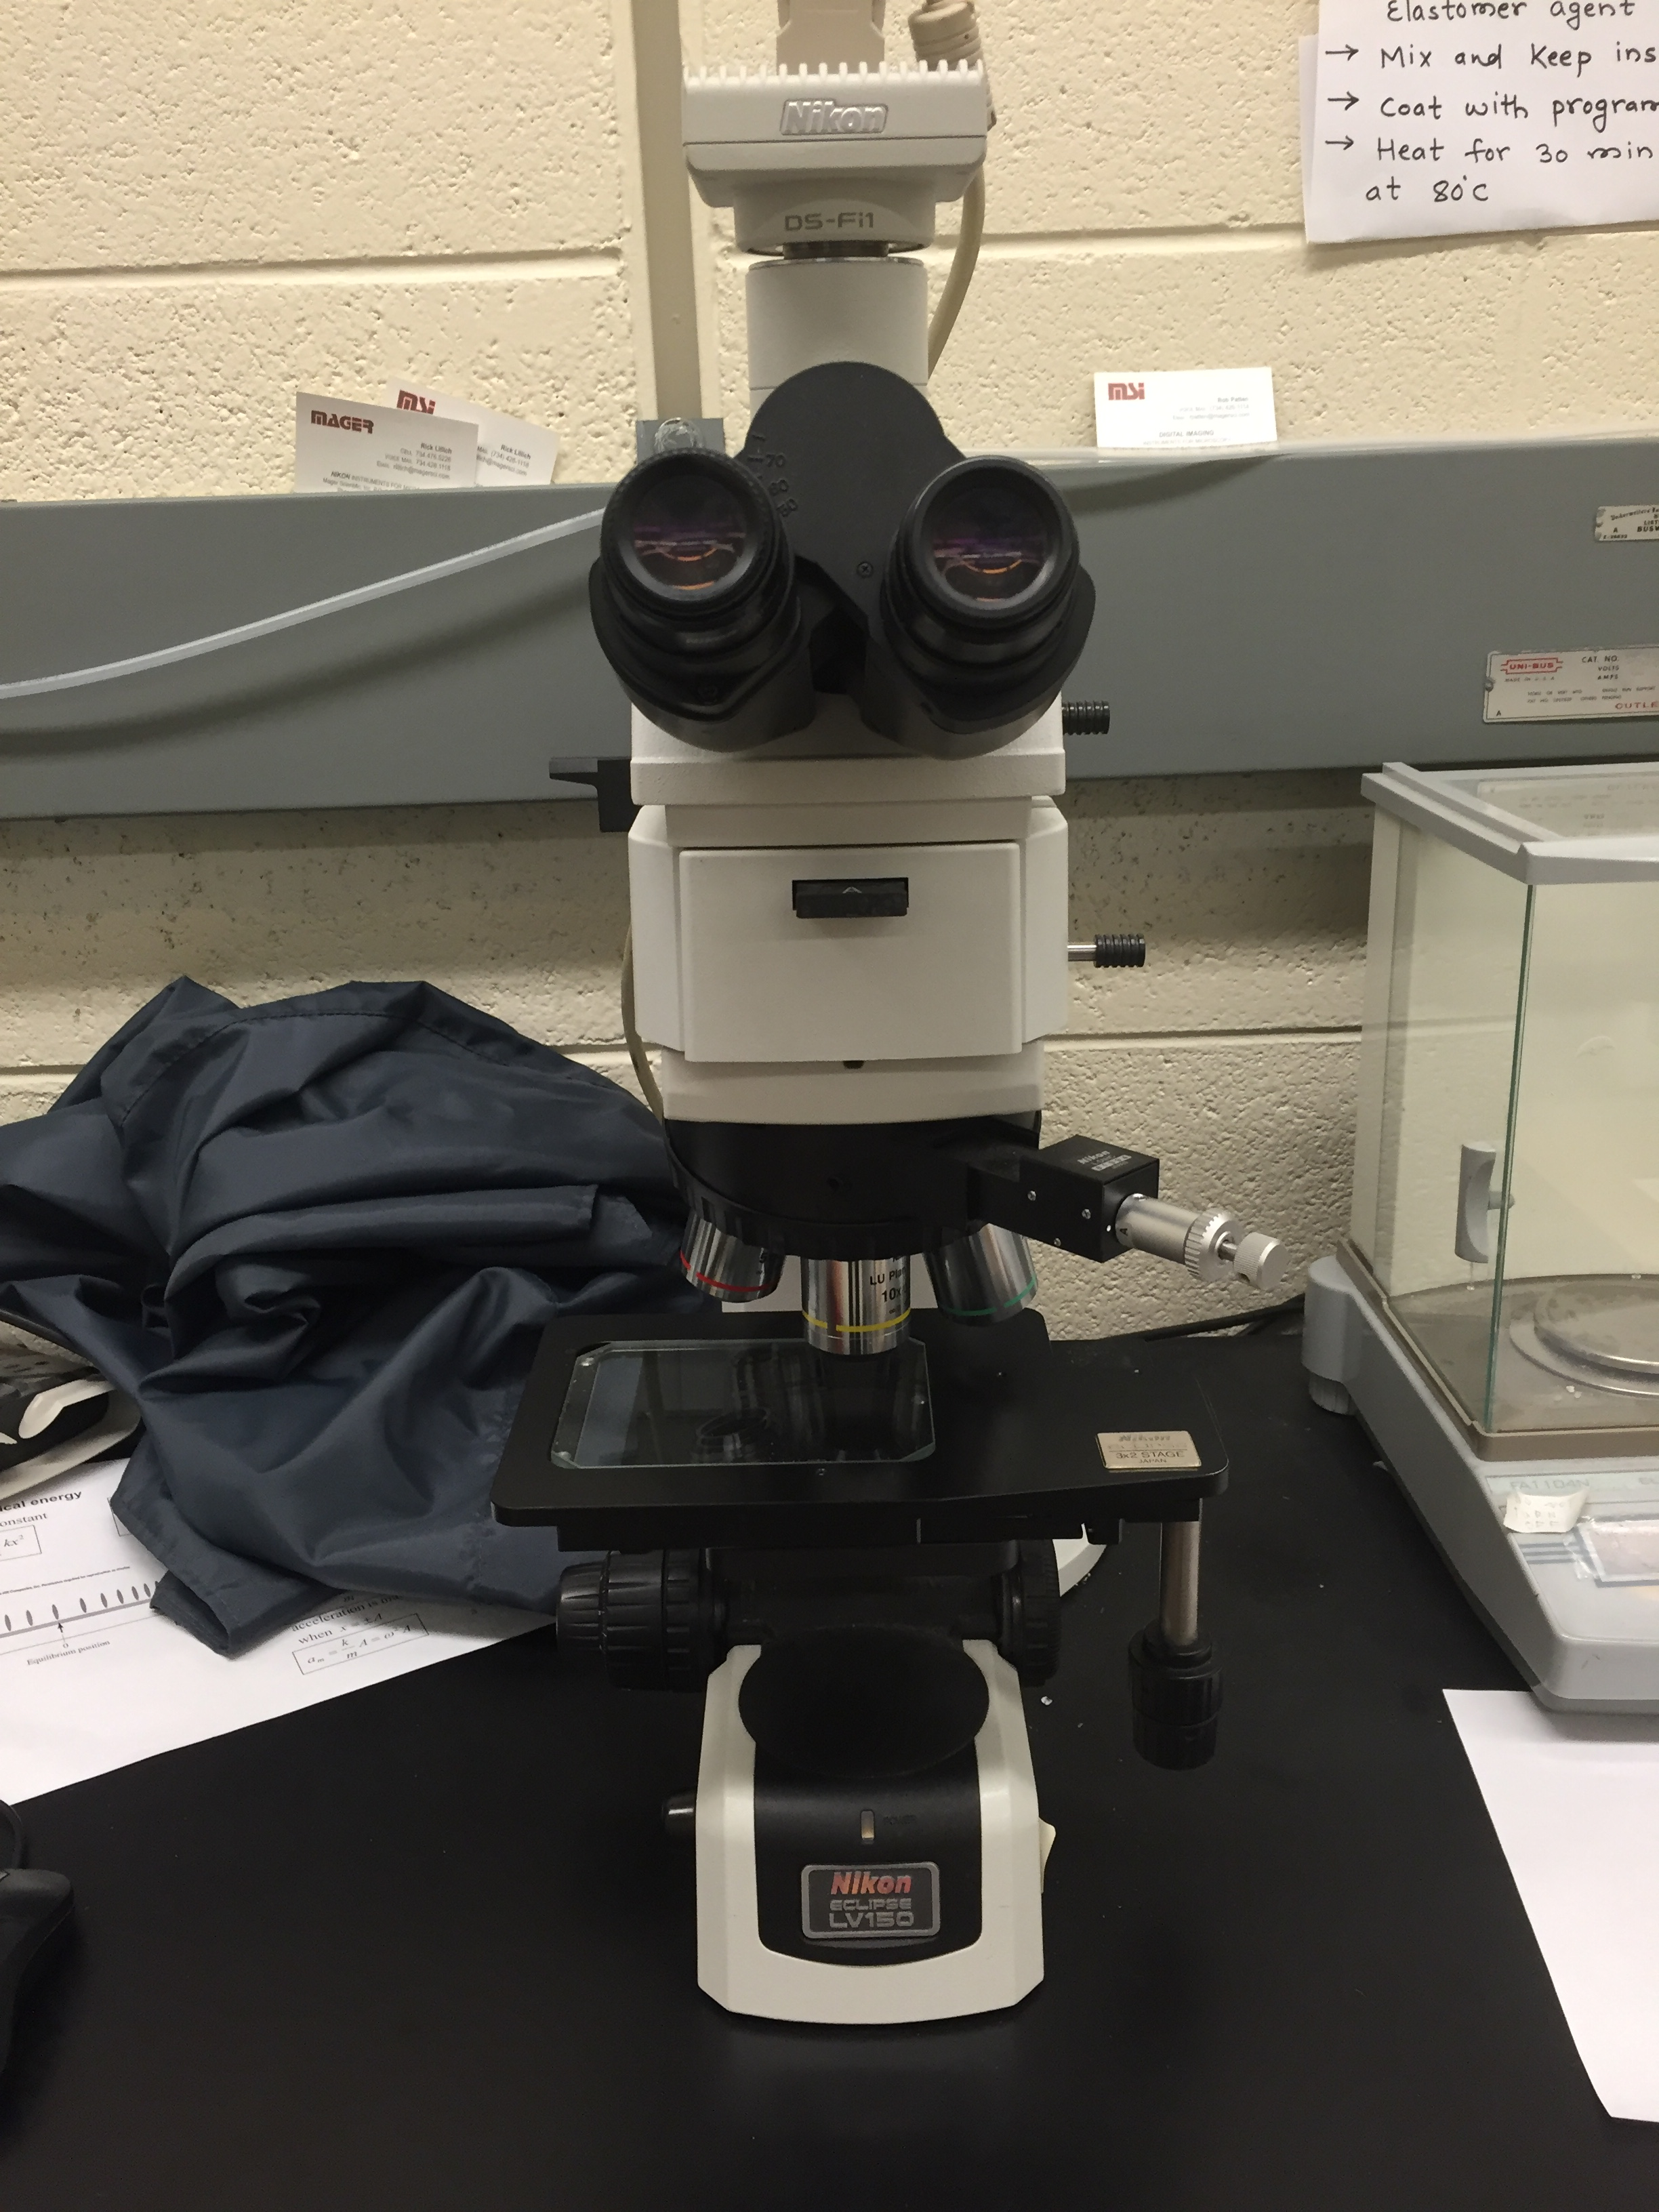
\includegraphics[height=5cm,width=3.5cm]{optical_microscope_front_view}
        \label{fig:optical_microscope_front_view}
    }
    \qquad
    \subfloat[]{
        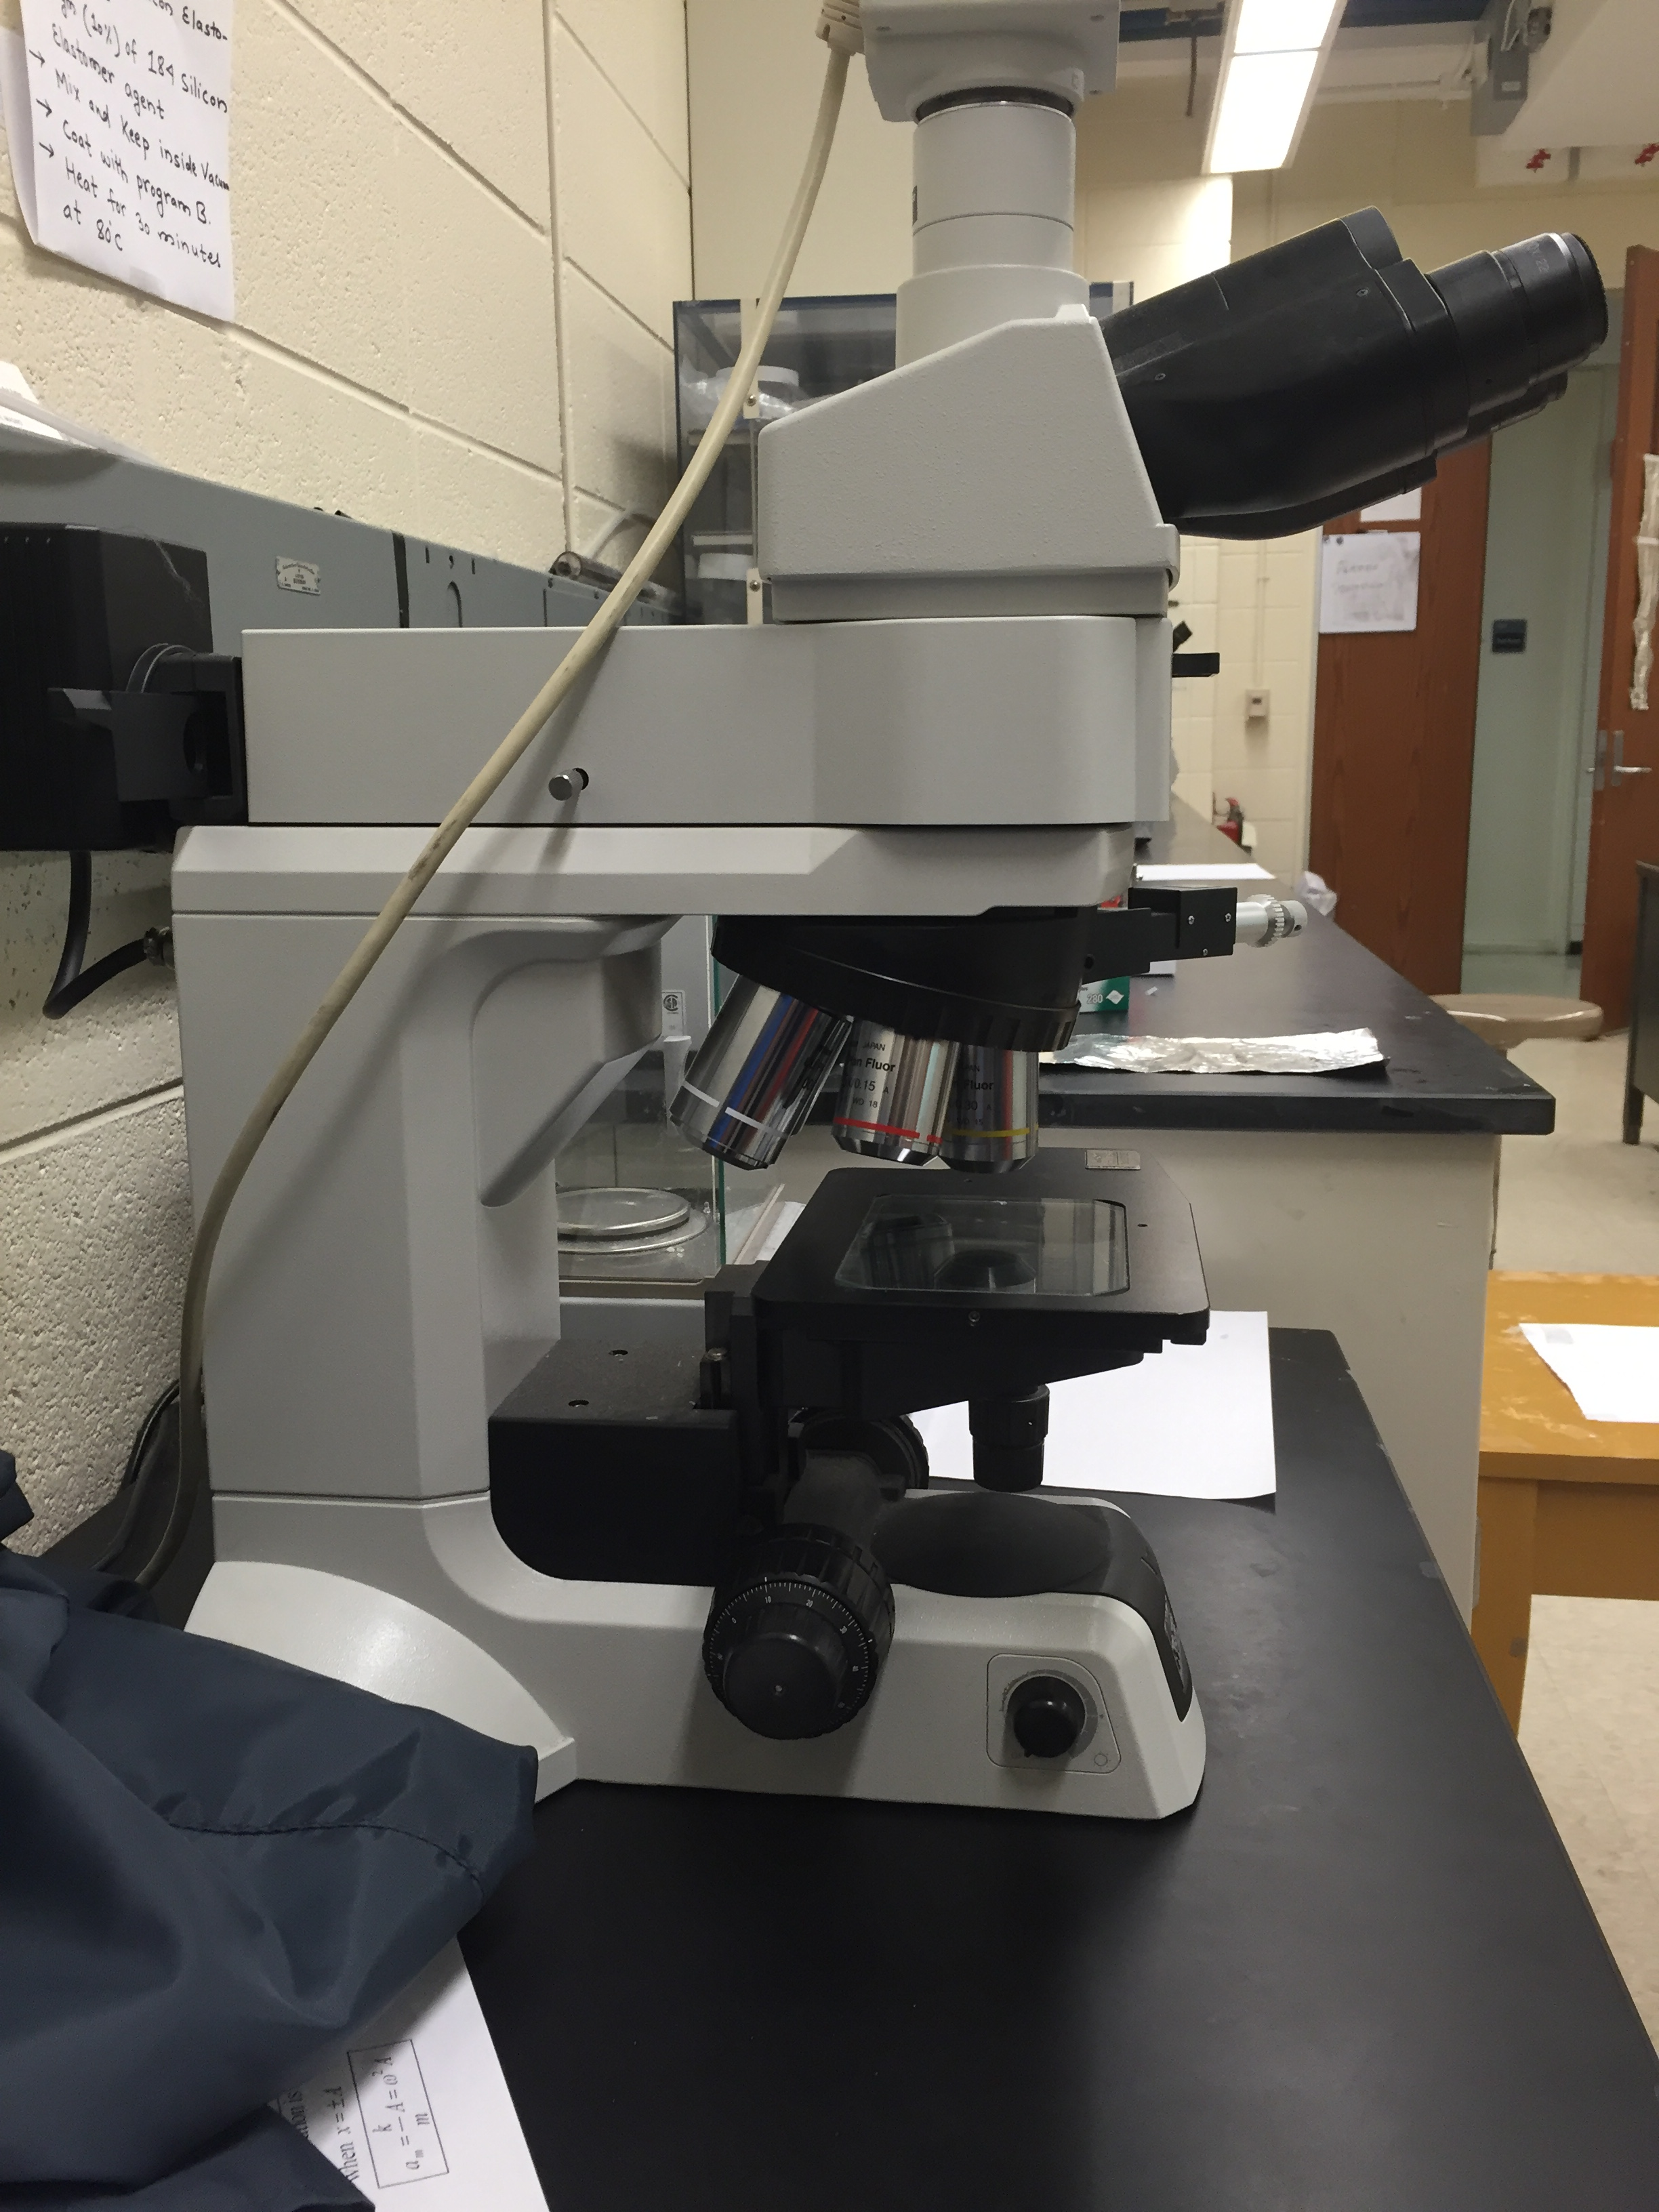
\includegraphics[height=5cm,width=3.5cm]{optical_microscope_side_view}
        \label{fig:optical_microscope_side_view}
    }
    \caption[Optical microscope setup]{
        Optical microscope setup with Nikon camera attachment.
        \protect\subref{fig:optical_microscope_front_view} Optical microscope front view. 
        \protect\subref{fig:optical_microscope_side_view} Optical microscope size view.}
\end{figure}
\begin{figure}[ht]
    \centering  
    \subfloat[]{
        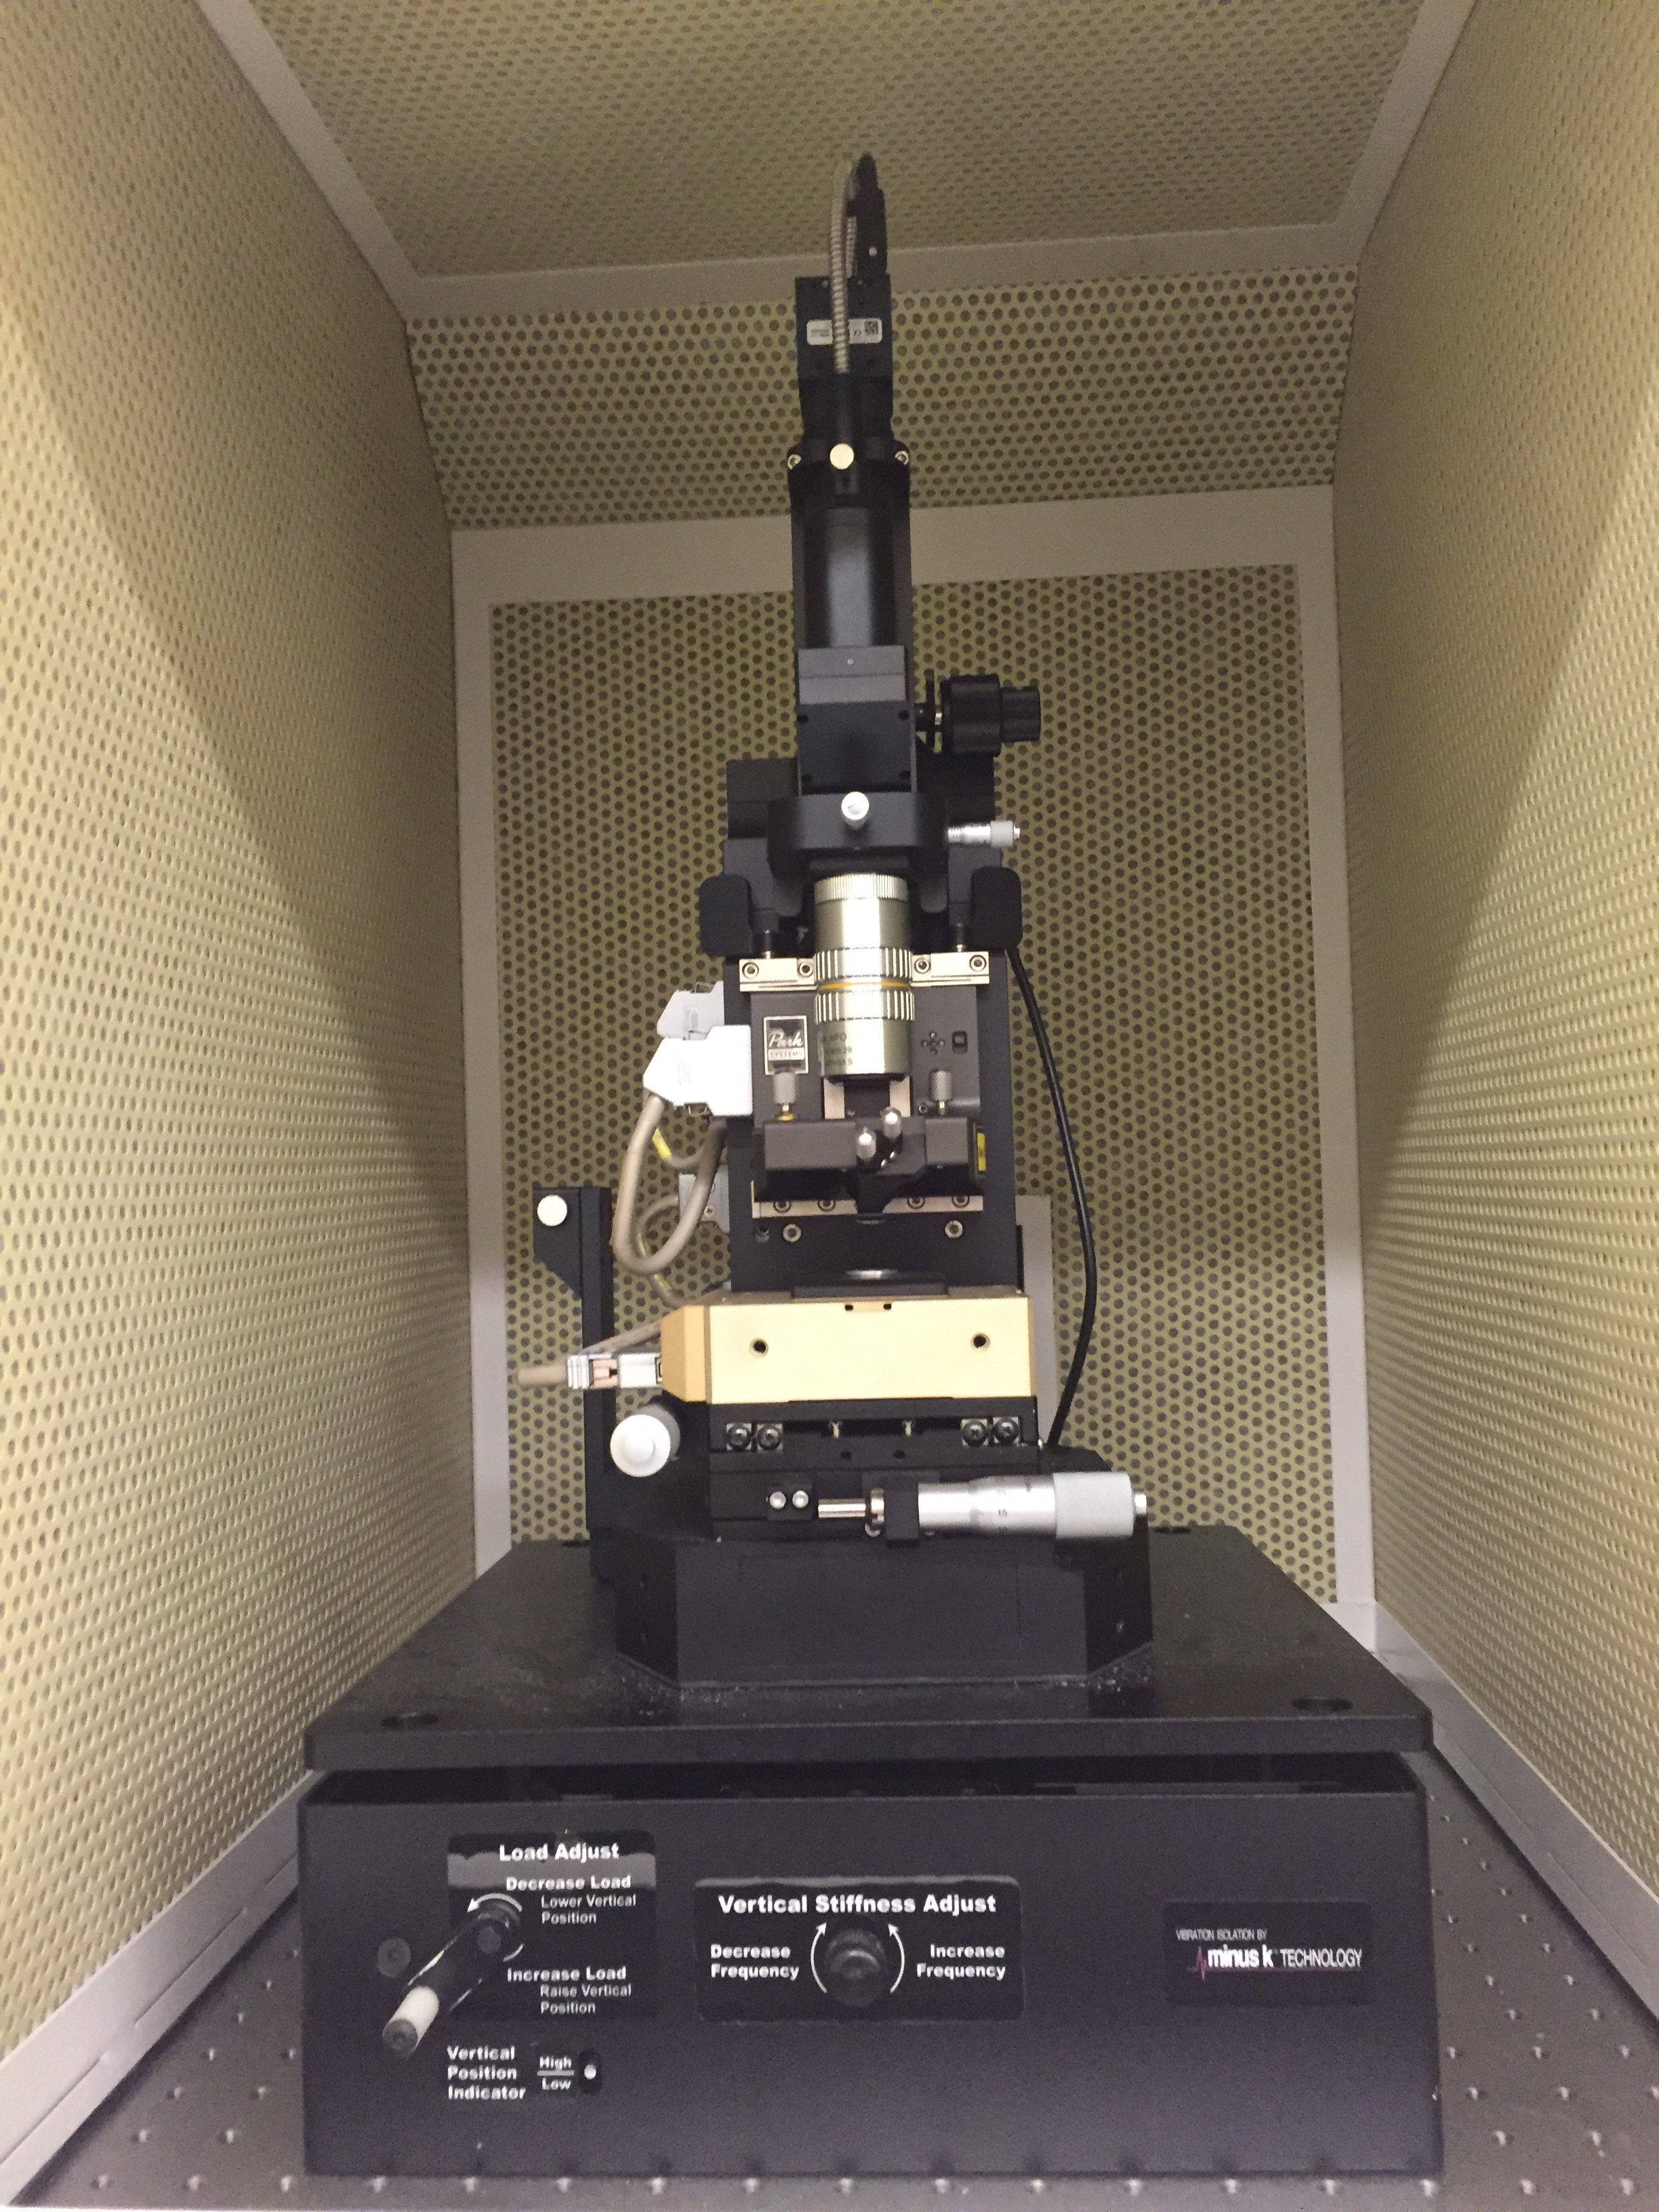
\includegraphics[height=4cm,width=4cm]{AFM_front_view}
        \label{fig:afm_front_view}
    }
    \qquad
    \subfloat[]{
        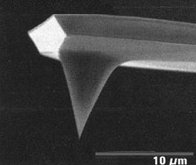
\includegraphics[height=4cm,width=4cm]{AFM_tip}
        \label{fig:AFM_tip}
    }
    \caption[Diagram of atomic force microscope setup and cantilever]{
        \acs{AFM} system setup with camera attachment. 
        \protect\subref{fig:afm_front_view} Front view of \acs{AFM} setup. 
        \protect\subref{fig:AFM_tip} AFM cantilever tip.
    }
\end{figure}

%--------------------------------------------------------------%
    % Transfer Methods
%--------------------------------------------------------------%
\section{Stacking and Assembly of Two-Dimensional Materials}\label{sec:transfer}

\begin{figure}[ht]
    \centering
    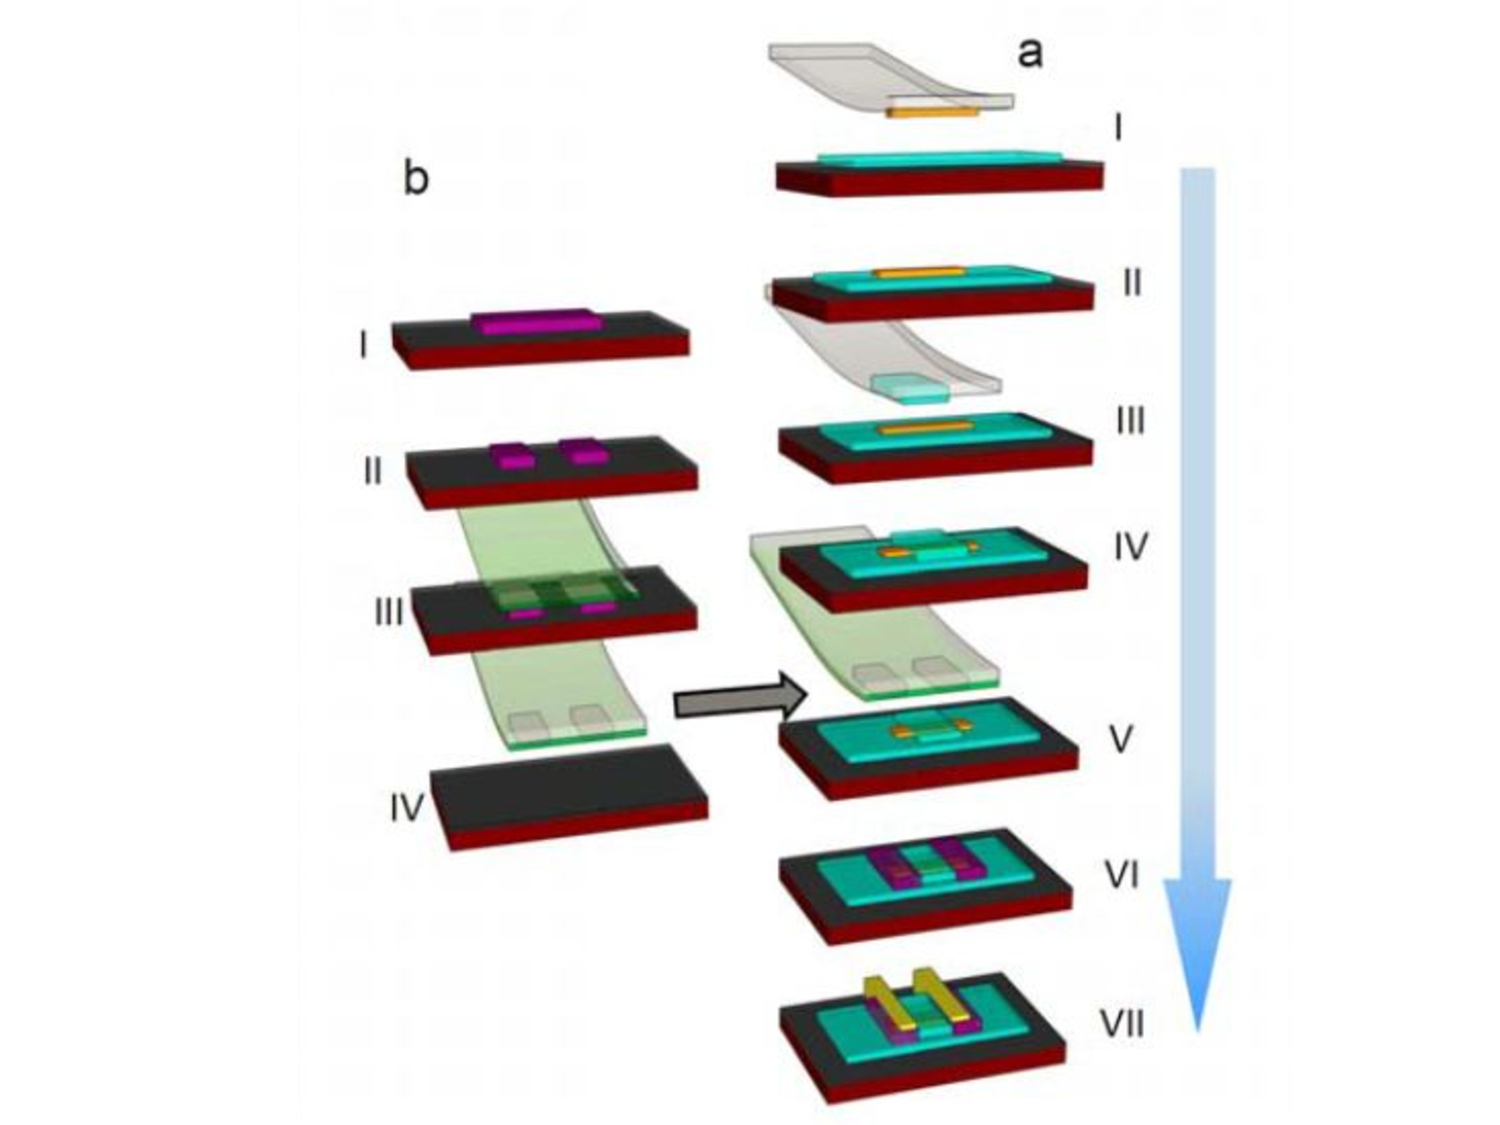
\includegraphics[height=10cm,width=10cm]{device_fab_diagram}
    \caption[Schematic and process flow of device fabrication using transfer techniques]
    {
        Caption.
    }
    \label{fig:device_fab_diagram}
\end{figure}

%--------------------------------------------------------------%
\subsection{PDMS Film Preparation}\label{subsec:pdms_prep}

%--------------------------------------------------------------%
\subsection{PDMS Transfer Method}\label{subsec:pdms_transfer}

\begin{figure}[ht]
    \centering
    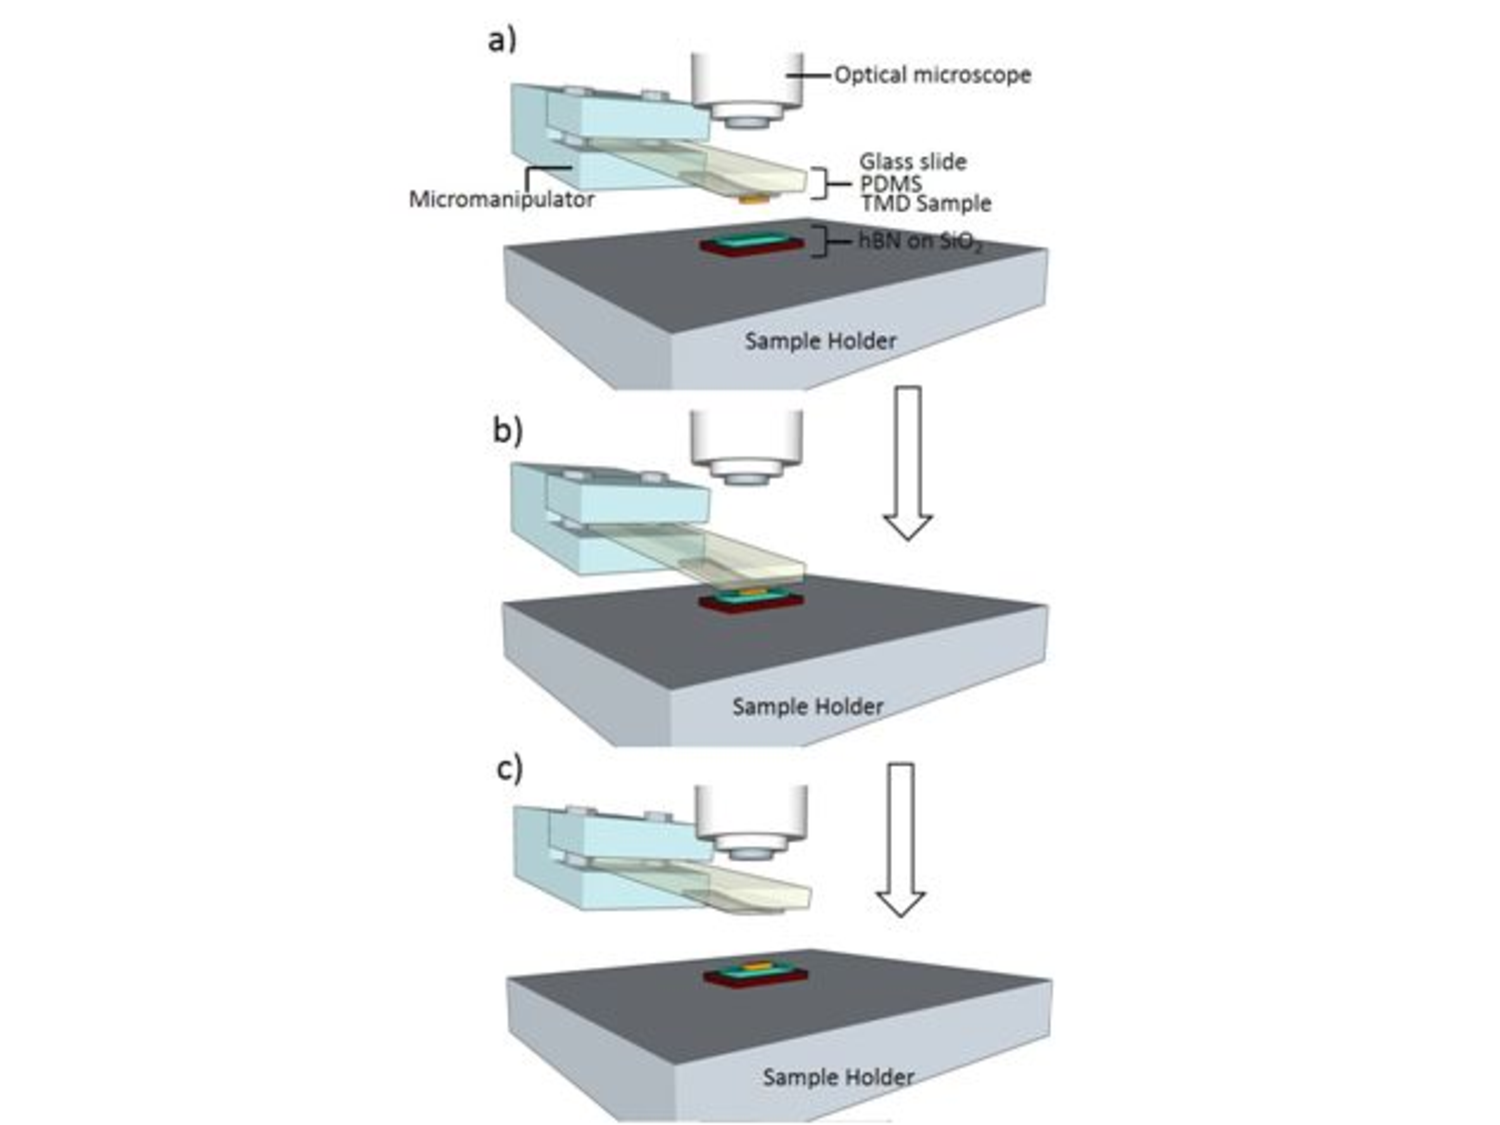
\includegraphics[height=10cm,width=14cm]{transfer_schematic}
    \caption[Schematic and process used for general \acs{PMDS} transfers]
    {
        Caption.
    }
    \label{fig:transfer_schematic}
\end{figure}

%--------------------------------------------------------------%
\subsection{PC Film Preparation}\label{subsec:pc_prep}

%--------------------------------------------------------------%
\subsection{Wet PC Transfer Method}\label{subsec:wet_pc_transfer}

\begin{figure}[ht]
    \centering
    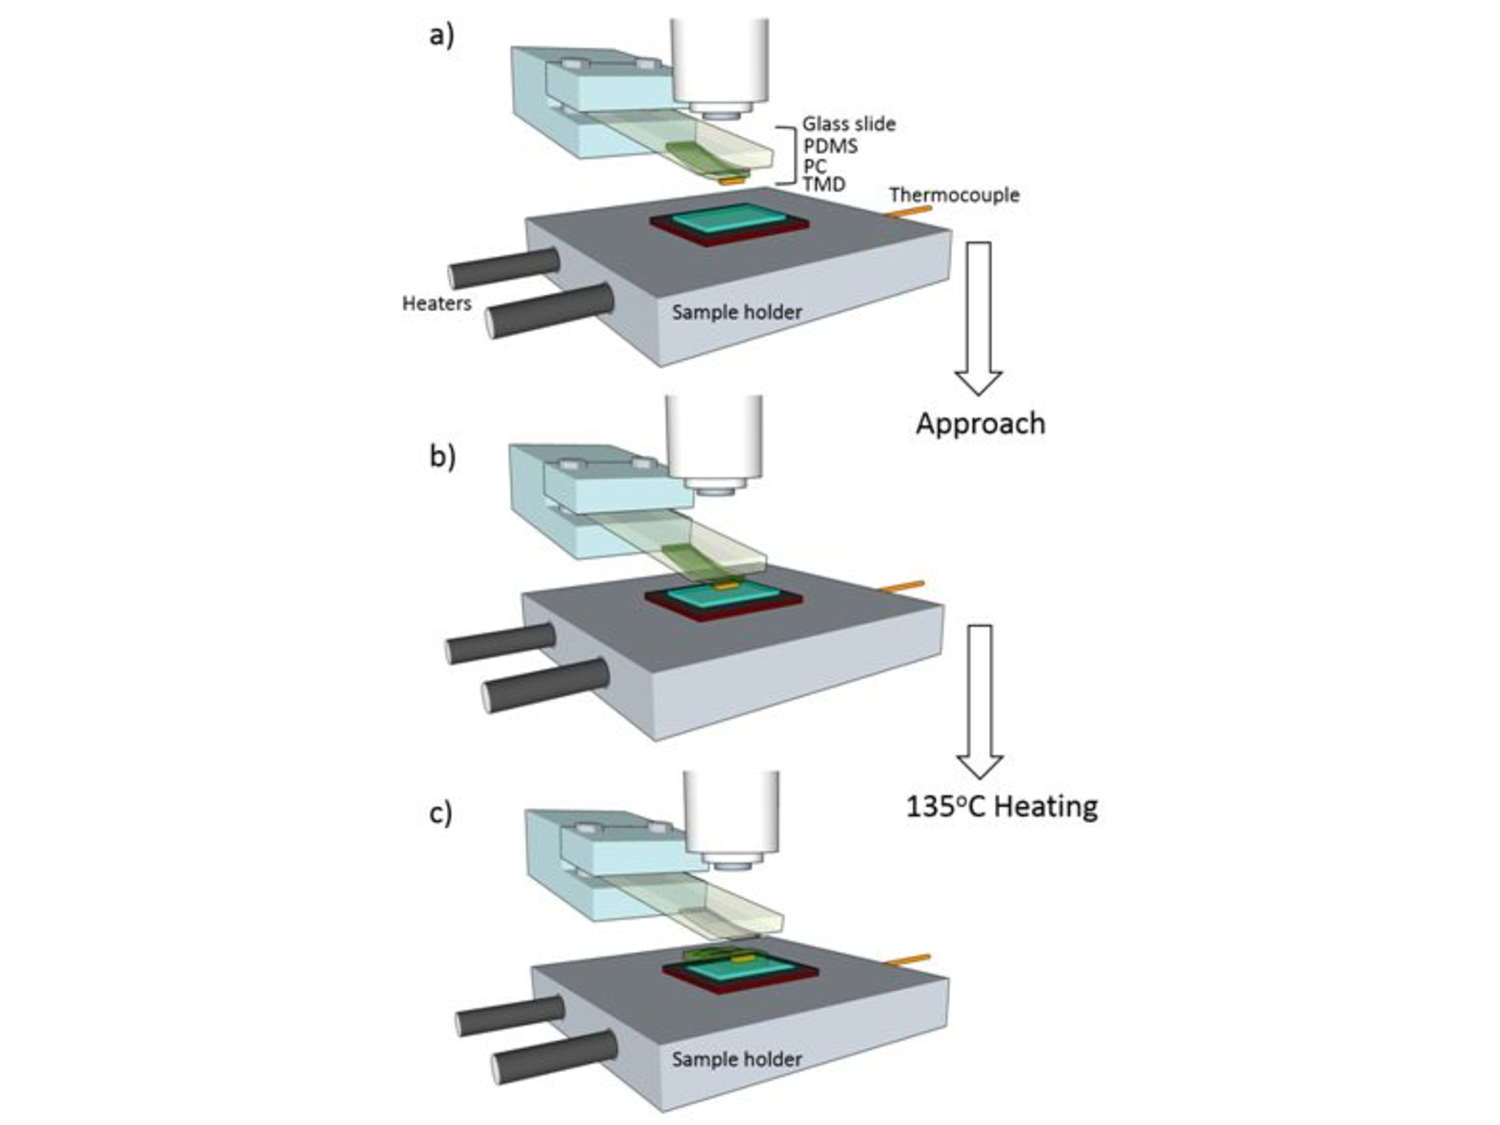
\includegraphics[height=10cm,width=14cm]{pickup_schematic}
    \caption[Schematic and process used for pickup transfers]
    {
        Caption.
    }
    \label{fig:pickup_schematic}
\end{figure}

%--------------------------------------------------------------%
\subsection{Dry PC Transfer and Sequential Pickup Methods}\label{subsec:dry_pc_transfer}

%--------------------------------------------------------------%
    % Doping Methods
%--------------------------------------------------------------%
%\section{Doping Methods}\label{sec:chemical_doping}

%--------------------------------------------------------------%
%\subsection{Doping Methods: Benzyl Viologen}\label{subsec:doping_bv}

%--------------------------------------------------------------%
%\subsection{Doping Methods: Polymer Electrolyte}\label{subsec:doping_pe}

%--------------------------------------------------------------%
    % General Fabrication Processes
%--------------------------------------------------------------%
\section{General Fabrication Processes}\label{sec:fab_processes}

%--------------------------------------------------------------%
\subsection{Electron Beam Lithography}\label{subsec:ebl}
\begin{figure}[ht]
    \centering
    \includegraphics[height=4cm,width=7cm]{SEM}
    \caption[Scanning electron microscope]{Control panel and electron beam writing system using a \acs{SEM}.}
    \label{fig:sem}
\end{figure} 

\begin{figure}[ht]
    \centering
    \subfloat[]{
        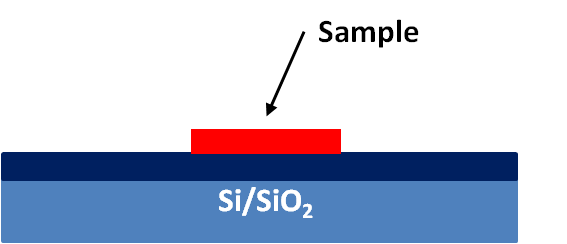
\includegraphics[height=3cm,width=5cm]{ebeam_step01}
        \label{fig:ebeam_step01}
    }
    \subfloat[]{
        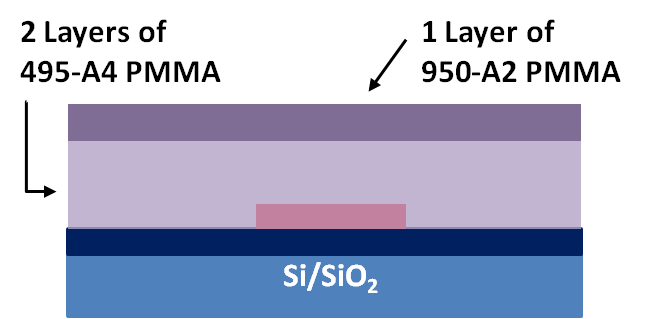
\includegraphics[height=3cm,width=5cm]{ebeam_step02}
        \label{fig:ebeam_step02}
    }
    \\
    \subfloat[]{
        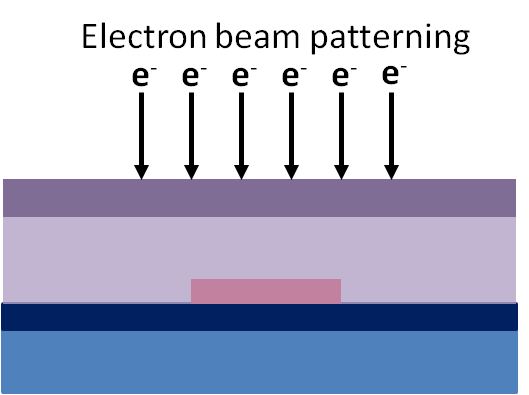
\includegraphics[height=3cm,width=5cm]{ebeam_step03}
        \label{fig:ebeam_step03}
    }
    \subfloat[]{
        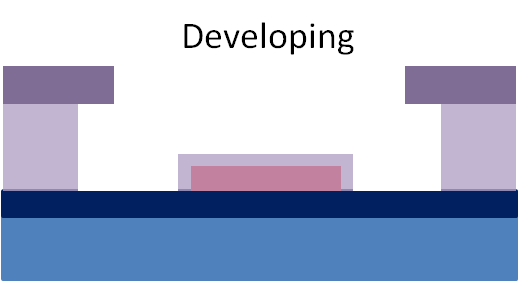
\includegraphics[height=3cm,width=5cm]{ebeam_step04}
        \label{fig:ebeam_step04}
    }
    \caption[Electron beam lithography steps and working principle]{
        The figure shows the working principle behind electron beam lithography and the purpose of applying multiple layers of \acs{PMMA} with different molecular weights. Since the bottom two layers 
        of \acs{PMMA} (495-A4) have a smaller molecular weight than the top layer of of \acs{PMMA} (950-A2) the cross-linking of \acs{PMMA} will be much easier for the electron beam
        to break resulting in an under-cut after developing.
        \protect\subref{fig:ebeam_step01} Shows the sample on a \ch{Si/SiO2} substrate before it is spin-coated with \acs{PMMA}. 
        \protect\subref{fig:ebeam_step02} The substrate and sample is shown spin-coated with two layers of \acs{PMMA} (495-A4) and one layer of \acs{PMMA} (950-A2).
        \protect\subref{fig:ebeam_step03} The \acs{PMMA} is bombarded with the electron beam.
        \protect\subref{fig:ebeam_step04} Upon developing the under-cut is shown, whereby the bottom two layers of \acs{PMMA} with smaller molecular weight has a wider area than the top, heavier molecular weight \acs{PMMA}.
    }
\end{figure}

\begin{figure}[ht]
    \centering 
    \subfloat[]{
        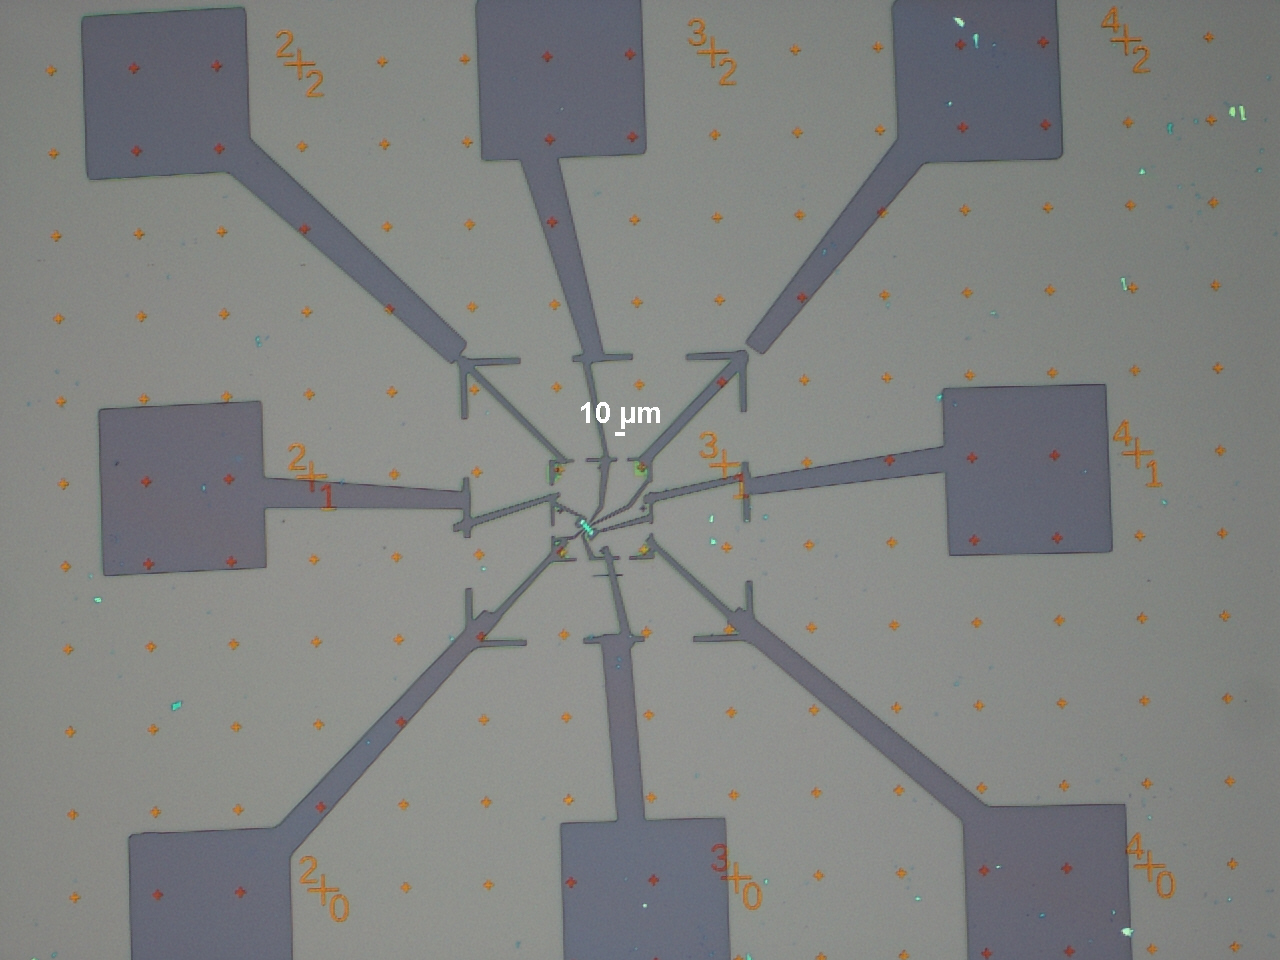
\includegraphics[height=5cm,width=6cm]{ebeam_developed_10x}
        \label{fig:ebeam_10x}
    }
    \qquad
    \subfloat[]{
        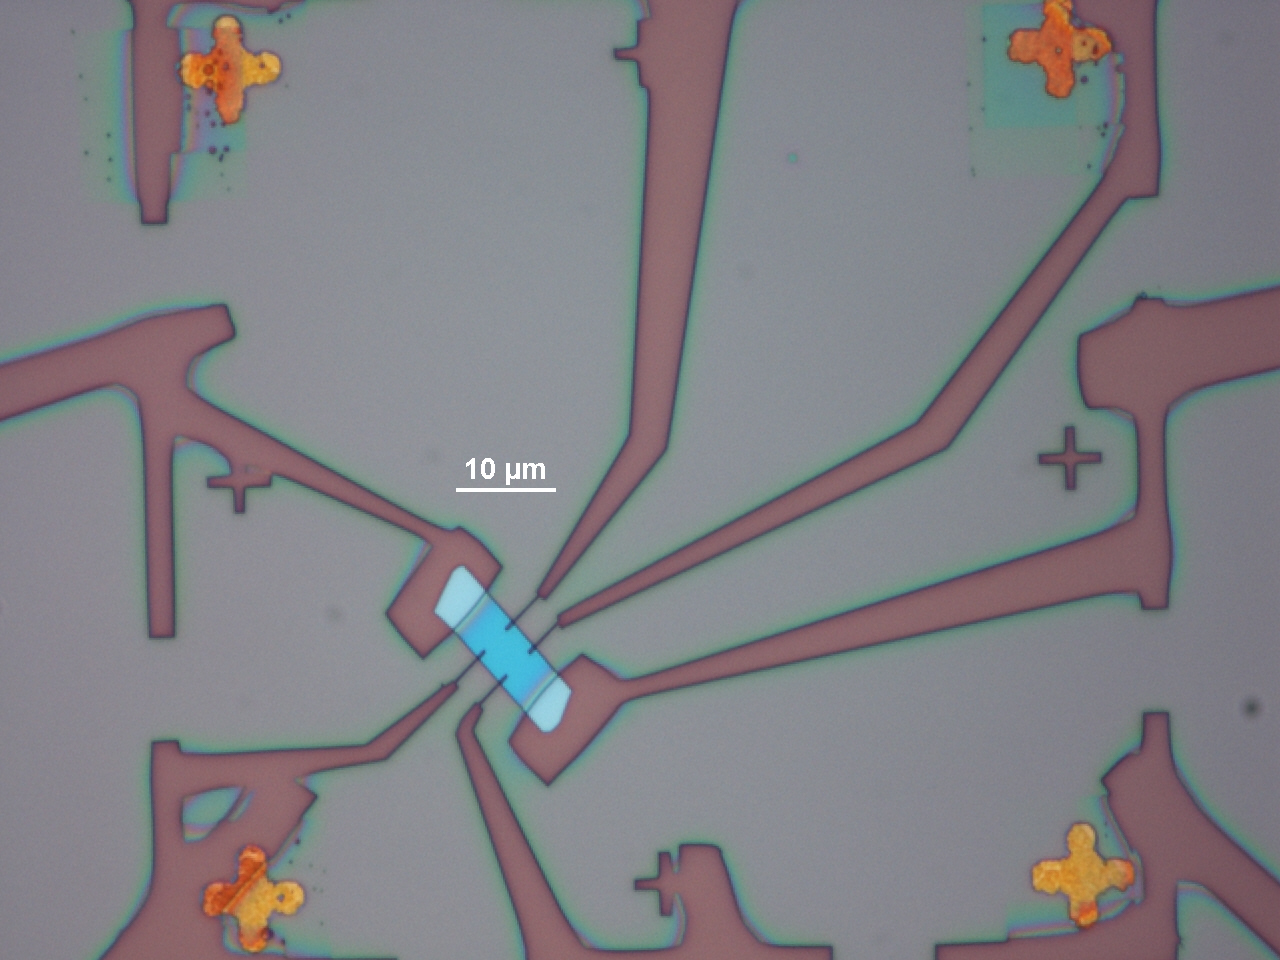
\includegraphics[height=5cm,width=6cm]{ebeam_developed_100x}
        \label{fig:ebeam_100x}
    }
    \caption[Example of electron beam lithography patterning]{
        Optical micrograph taken after \acs{EBL} and developing described in \ref{fig:ebeam_step03} and \ref{fig:ebeam_step04}.
        \protect\subref{fig:ebeam_10x} Shows the pattern on after developing taken under 10x magnification.
        \protect\subref{fig:ebeam_100x} Is an enlarged micrograph shown at 100x magnification. The pink color contrast shows the area where \acs{EBL} was patterned and the outer area that do not have a 
        pink contrast shows where \acs{PMMA} still remains. In this case the device was patterned for a four probe measurement.
    }
\end{figure}

%--------------------------------------------------------------%
\subsection{Photolithography}\label{subsec:photo_lithography}

\begin{figure}[ht]
    \centering
    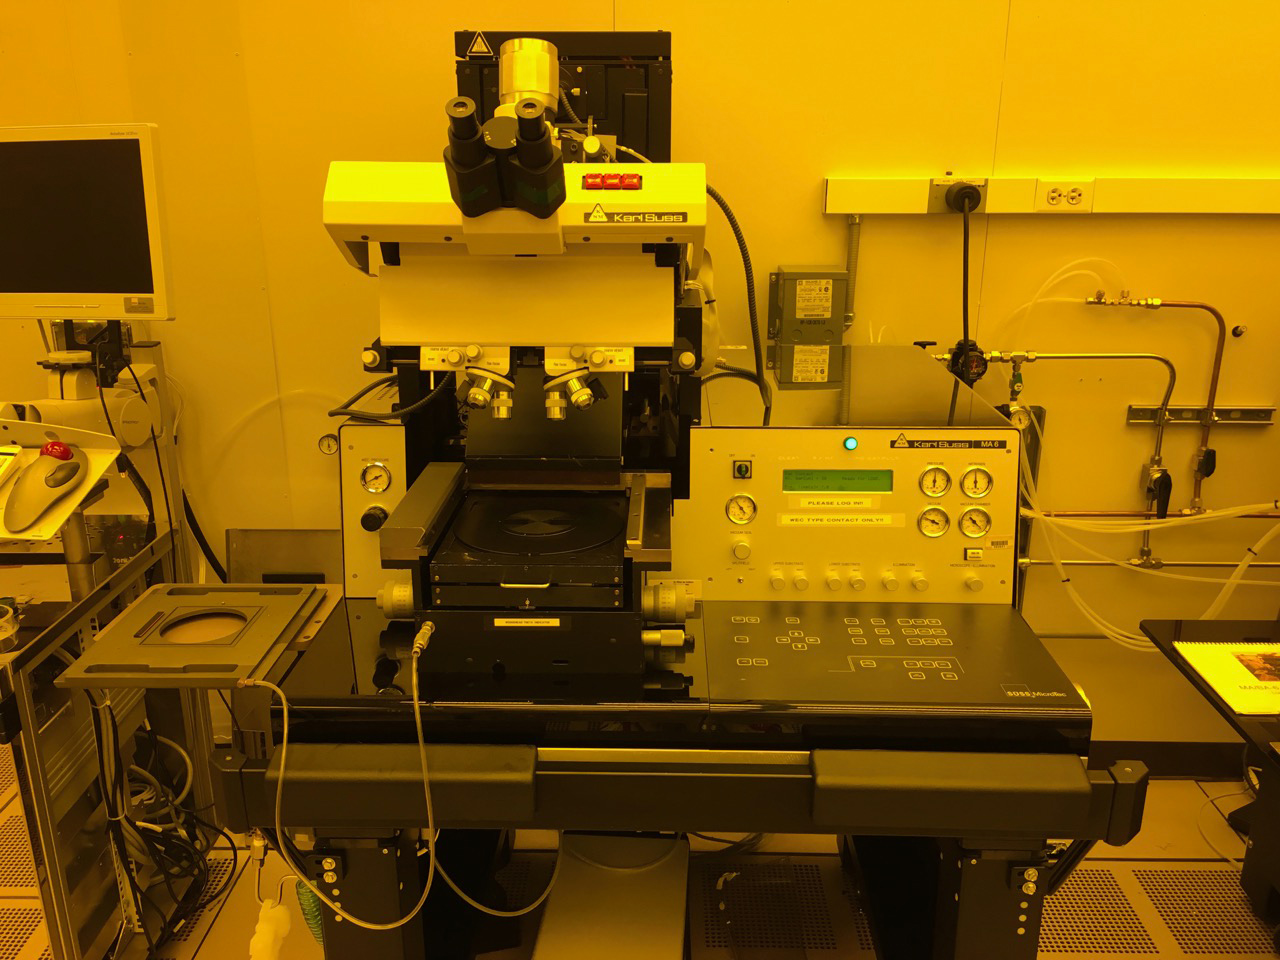
\includegraphics[height=5cm,width=7cm]{mask_aligner}
    \caption[Mask aligner for photolithography]{}
    \label{fig:mask_aligner}
\end{figure}

%--------------------------------------------------------------%
\subsection{Metal Deposition}\label{subsec:metal_deposition}

\begin{figure}[ht]
    \centering
    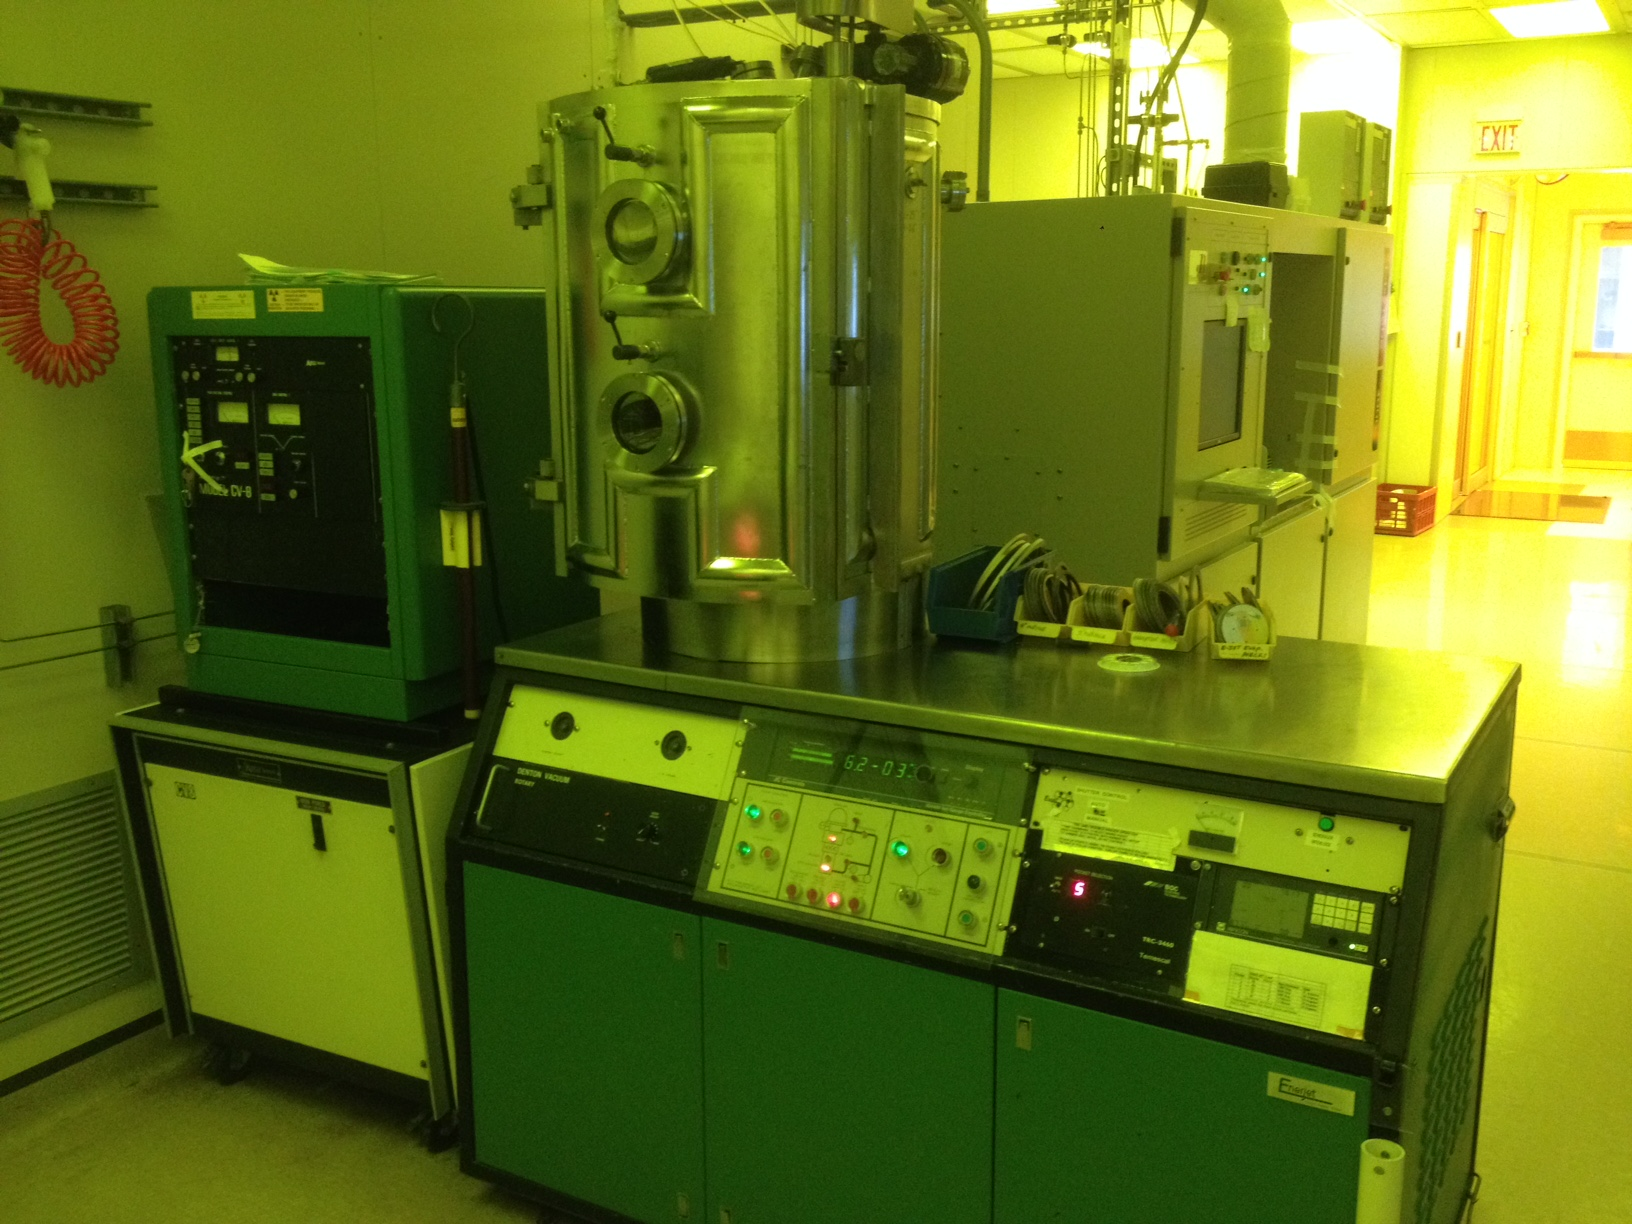
\includegraphics[height=5cm,width=8cm]{enerjet}
    \caption[Metal deposition system]{}
    \label{fig:enerjet}
\end{figure}

%--------------------------------------------------------------%
\subsection{Lift Off}\label{subsec:lift_off}

\begin{figure}[ht]
    \centering 
    \subfloat[]{
        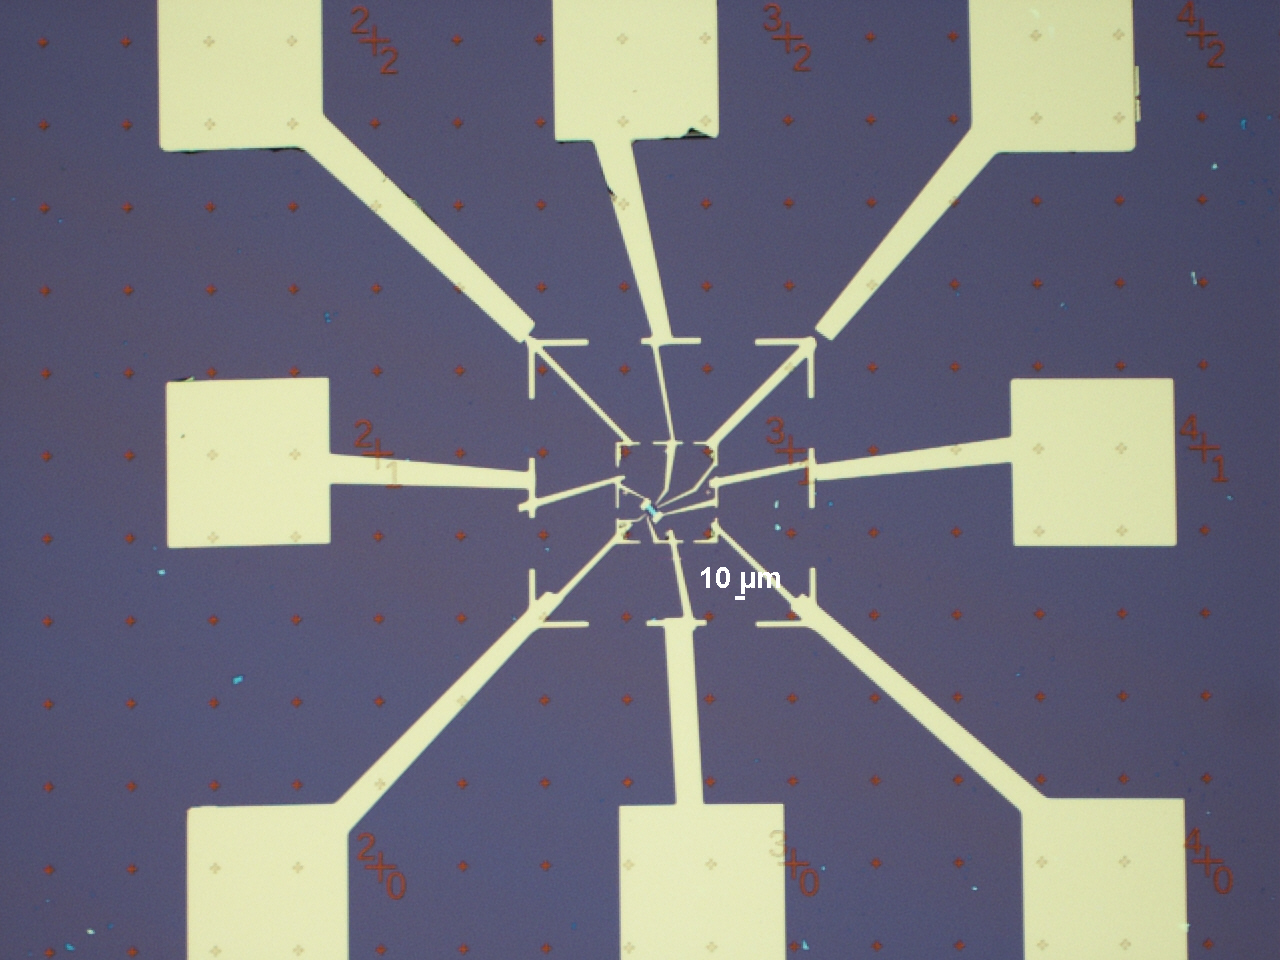
\includegraphics[height=5cm,width=6cm]{liftoff_10x}
        \label{fig:liftoff_10x}
    }
    \qquad
    \subfloat[]{
        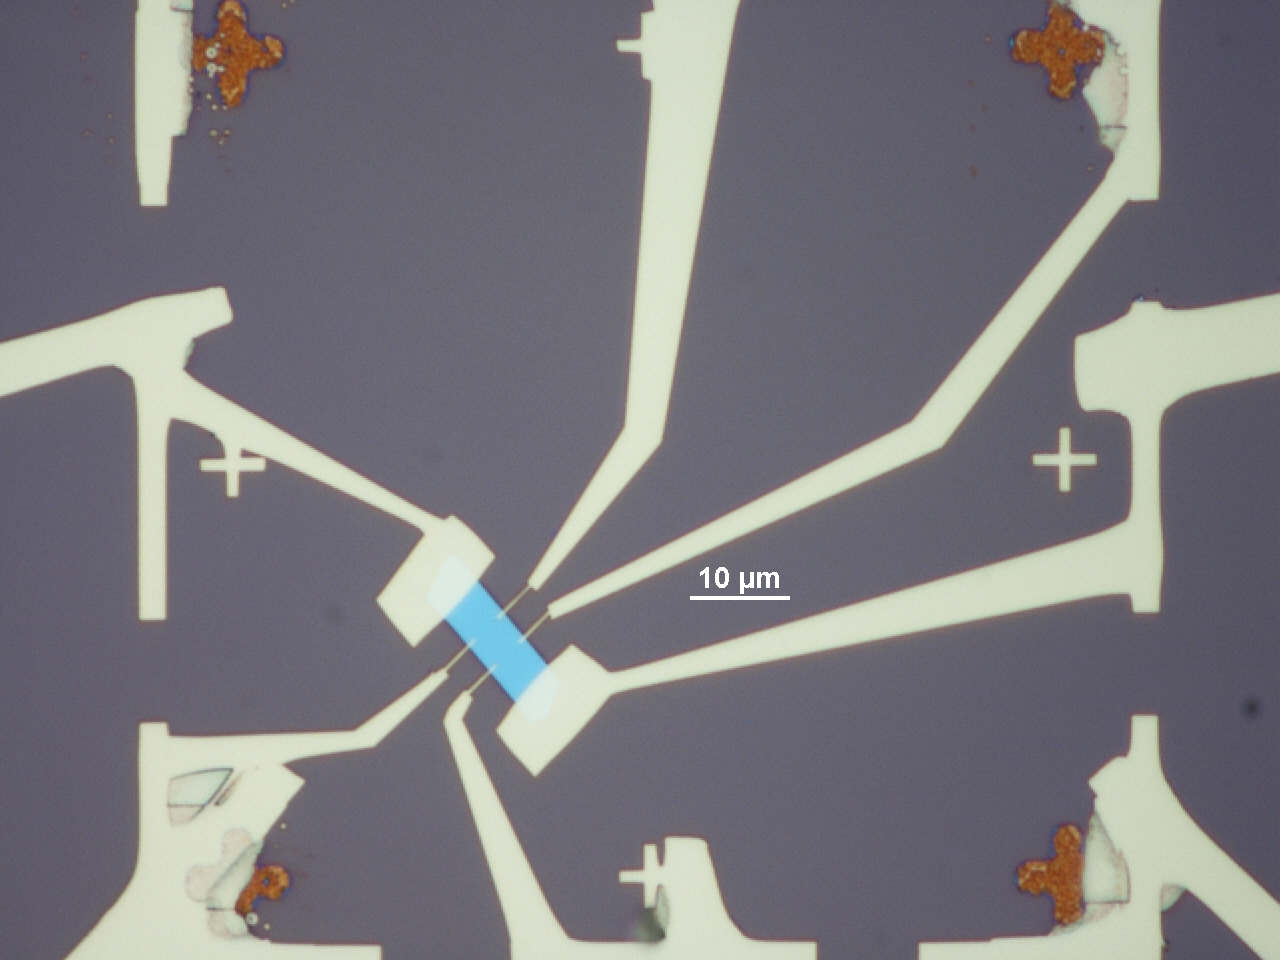
\includegraphics[height=5cm,width=6cm]{liftoff_100x}
        \label{fig:liftoff_100x}
    }
    \caption[Example of electrodes after liftoff]{
        Optical micrograph taken after metal deposition and liftoff. 
        \protect\subref{fig:liftoff_10x} Shows an image taken under 10x magnification. This image corresponds to the developed pattern shown in \ref{fig:ebeam_10x}.
        \protect\subref{fig:liftoff_100x} An enlarged image of the device under 100x magnification corresponding to the developed pattern shown in \ref{fig:ebeam_100x}.
    }
\end{figure}

%--------------------------------------------------------------%
\subsection{Sample Annealing}\label{subsec:annealing}
\begin{figure}[ht]
    \centering
    \subfloat[]{
        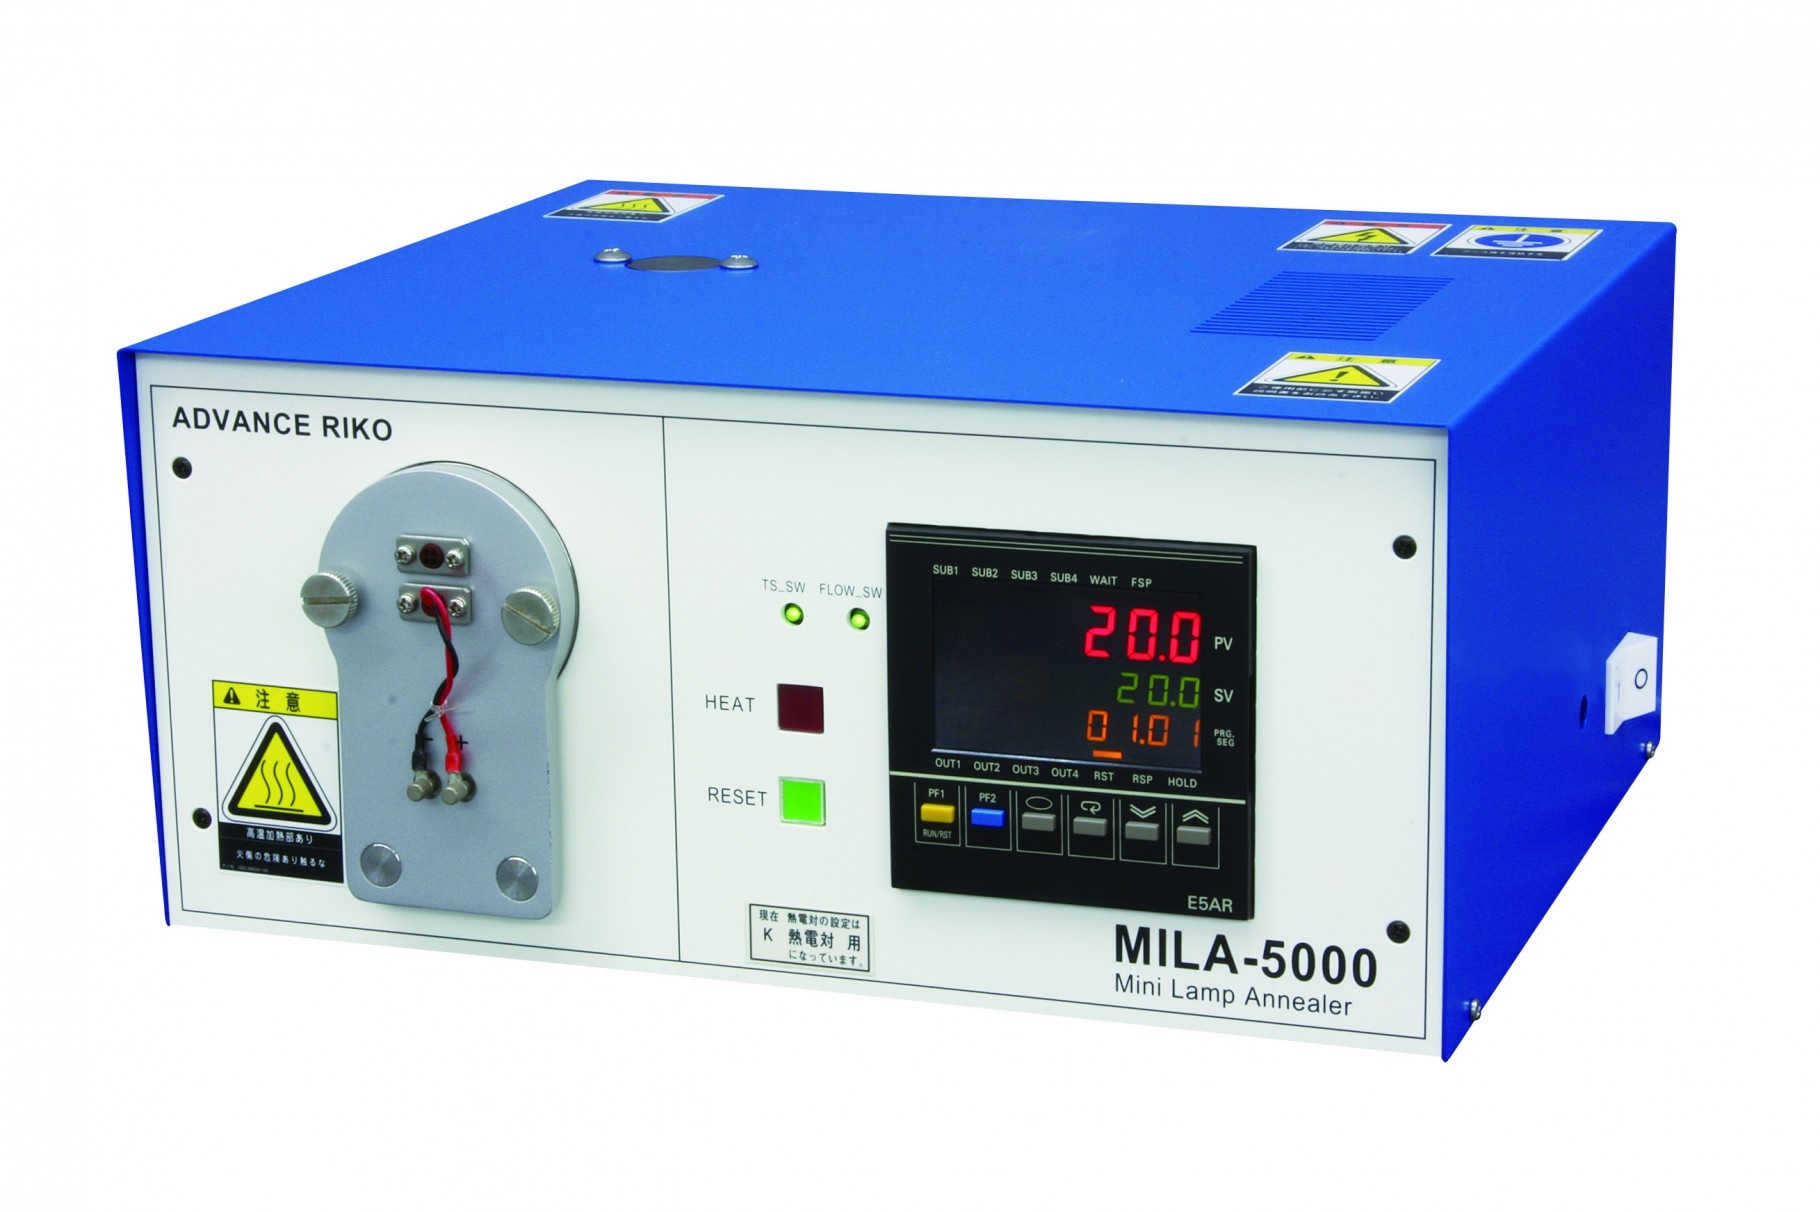
\includegraphics[height=6cm,width=8.5cm]{annealer}
        \label{fig:annealer}
    }
    \subfloat[]{
        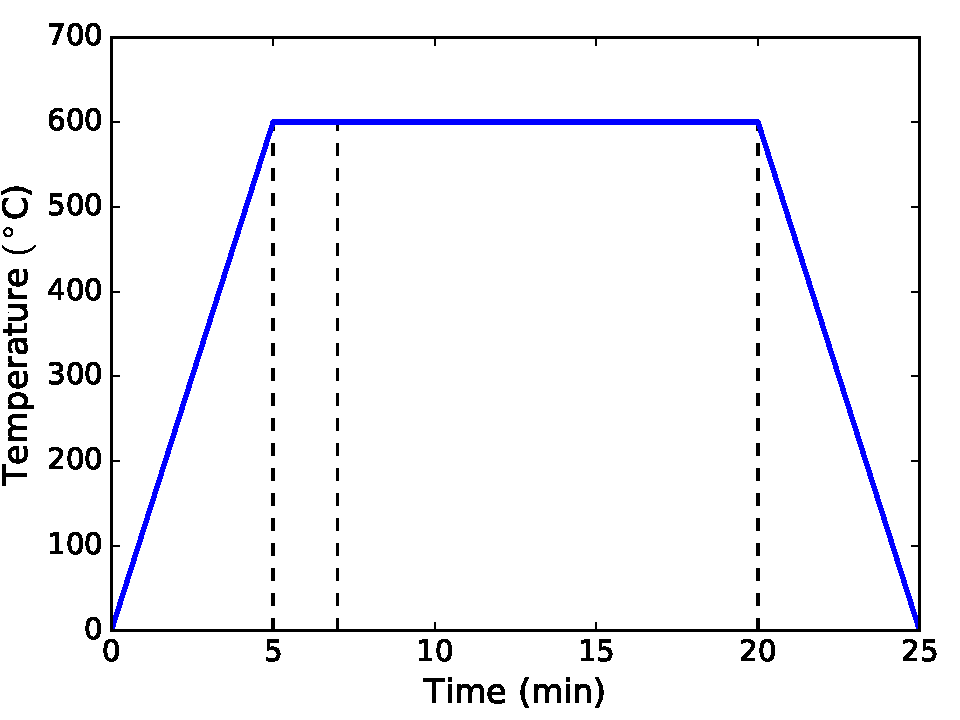
\includegraphics[height=5.5cm,width=7.5cm]{annealed_program06_plot}
        \label{fig:prog06_anneal}
    }
    \qquad
    \subfloat[]{
        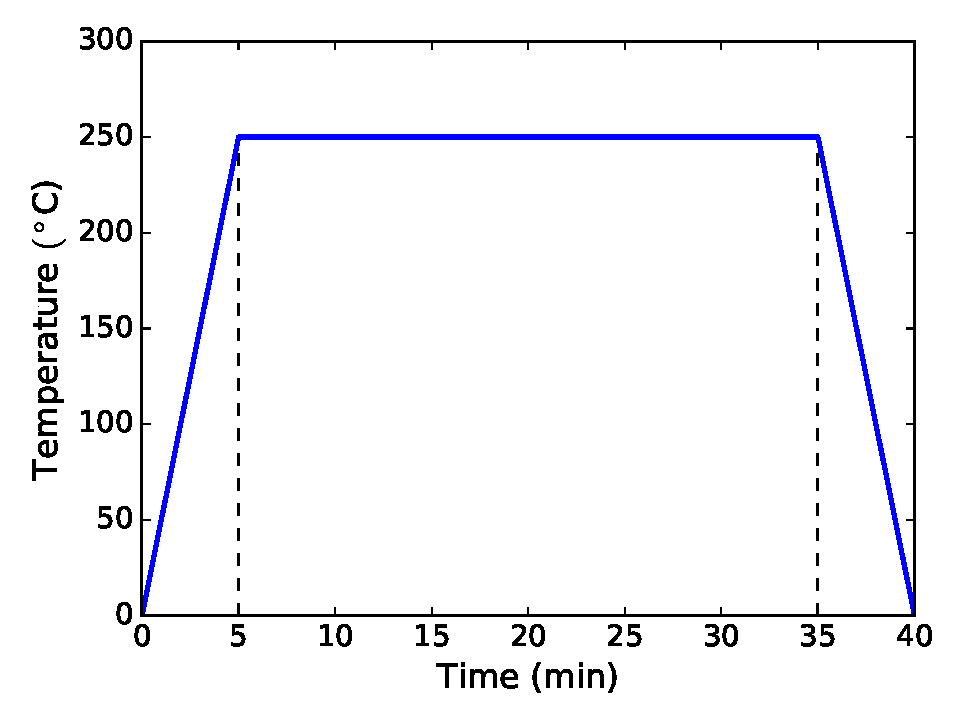
\includegraphics[height=5.5cm,width=7.5cm]{annealed_program03_plot}
        \label{fig:prog03_anneal}
    }
    \caption[Annealing equipment and annealing program temperature as a function of time]{
        \protect\subref{fig:annealer} The annealing equipment setup. 
        \protect\subref{fig:prog06_anneal} The temperature as a function of time for program number 6. In this case the dashed line at five minutes indicates the beginning of the forming gas phase of the process, the dashed line at seven minutes indicates the end of the forming gas phase, and the line at 25 minutes indicates the beginning of the cooling phase.
        \protect\subref{fig:prog03_anneal} The temperature as a function of time for program number 3. The dashed lines at 5 and 35 minutes indicates the end of the heating phase and beginning of the cooling phase, respectively. 
    }
\end{figure}

%--------------------------------------------------------------%
    % End of Chapter
%--------------------------------------------------------------%